\subsubsection*{Aspectos cuantitativos}

\begin{figure}[H]
    \centering
    \begin{tikzpicture}
        \pie[text=legend]{
            30.77/Menos de 2 veces al mes, 26.92/No sabía que había una aplicación o\dots, 19.23/Un día a la semana, 19.23/Menos de 4 días a la semana, 3.85/Más de 4 días a la semana
        }
    \end{tikzpicture}
    \caption{¿Cada cuánto usas la aplicación de la liga de la UIB o consultas la información de la liga a través de ella?}
    \label{fig:col_use}
\end{figure}
\begin{figure}[H]
    \centering
    \begin{tikzpicture}
        \pie[text=legend]{
            38.46/Aplicación móvil, 34.62/Navegador web, 26.92/No accedo
        }
    \end{tikzpicture}
    \caption{¿A través de qué medio accedes principalmente a la aplicación?}
    \label{fig:col_device}
\end{figure}

\subsubsection*{Aspectos cualitativos}


\begin{figure}[H]
    \centering
    \pgfplotsset{
        % Configuración ajustada con más separación en Título y Eje X
        tight grid bar/.style={
            width=\linewidth,
            height=5.8cm,
            ybar,
            bar width=10pt,
            xlabel={Puntuación},
            ylabel={Número de votos},
            % Separación de etiquetas respecto al marco
            xlabel style={yshift=-0.2em},      % Aleja la etiqueta del eje X hacia abajo
            ylabel style={yshift=-0.6em},      % Mantiene el eje Y intacto
            title style={yshift=0.5em},        % Eleva el título hacia arriba
            % Elimina el margen exterior que reserva pgfplots para etiquetas
            trim axis left,
            trim axis right,
            nodes near coords, 
            nodes near coords align={vertical},
            every node near coord/.append style={
                font=\small,
                /pgf/number format/.cd, fixed, precision=0
            },
            enlarge x limits=0.08,
            enlarge y limits={upper, value=0.15}
        }
    }

    \begin{subfigure}{0.49\textwidth}
        \centering
        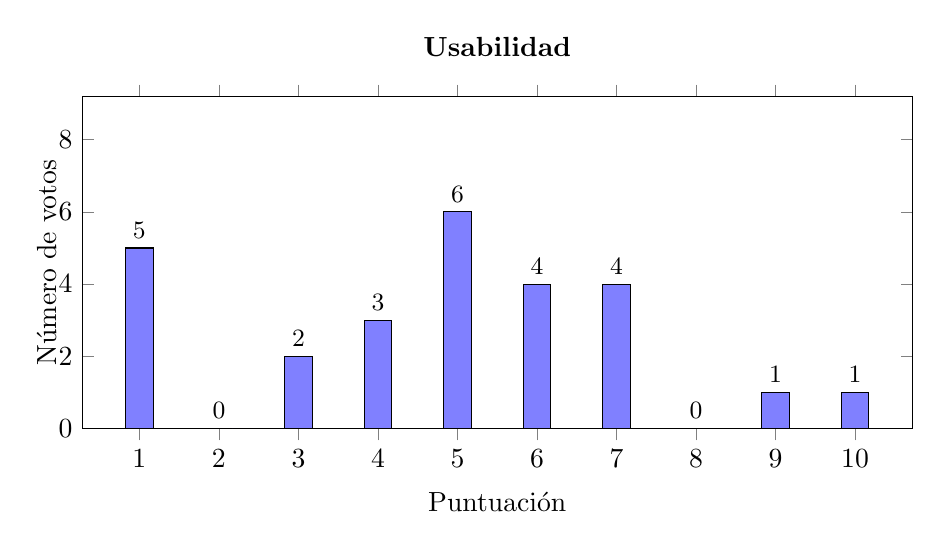
\begin{tikzpicture}
            \begin{axis}[
                tight grid bar,
                title={\textbf{Usabilidad}},
                ymin=0, ymax=8,
                ytick={0, 2, 4, 6, 8},
                xtick={1, 2, 3, 4, 5, 6, 7, 8, 9, 10},
                symbolic x coords={1, 2, 3, 4, 5, 6, 7, 8, 9, 10}
            ]
            \addplot[fill=blue!50] coordinates {
                (1, 5) (2, 0) (3, 2) (4, 3) (5, 6) (6, 4) (7, 4) (8, 0) (9, 1) (10, 1)
            };
            \end{axis}
        \end{tikzpicture}
    \end{subfigure}\hfill
    \begin{subfigure}{0.49\textwidth}
        \centering
        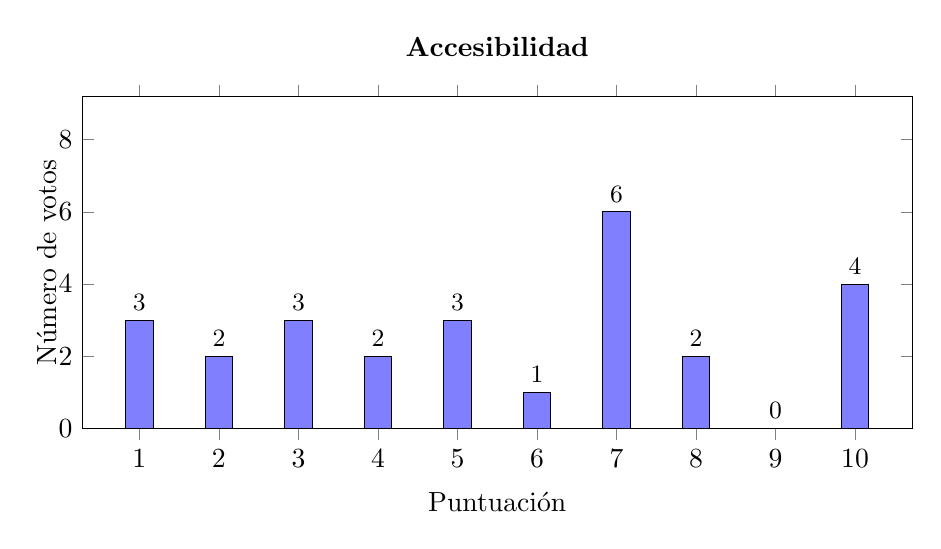
\begin{tikzpicture}
            \begin{axis}[
                tight grid bar,
                title={\textbf{Accesibilidad}},
                ymin=0, ymax=8,
                ytick={0, 2, 4, 6, 8},
                xtick={1, 2, 3, 4, 5, 6, 7, 8, 9, 10},
                symbolic x coords={1, 2, 3, 4, 5, 6, 7, 8, 9, 10}
            ]
            \addplot[fill=blue!50] coordinates {
                (1, 3) (2, 2) (3, 3) (4, 2) (5, 3) (6, 1) (7, 6) (8, 2) (9, 0) (10, 4)
            };
            \end{axis}
        \end{tikzpicture}
    \end{subfigure}

    \vspace{0.4cm} % Ligero incremento de separación entre filas por el desplazamiento del título inferior

    \begin{subfigure}{0.49\textwidth}
        \centering
        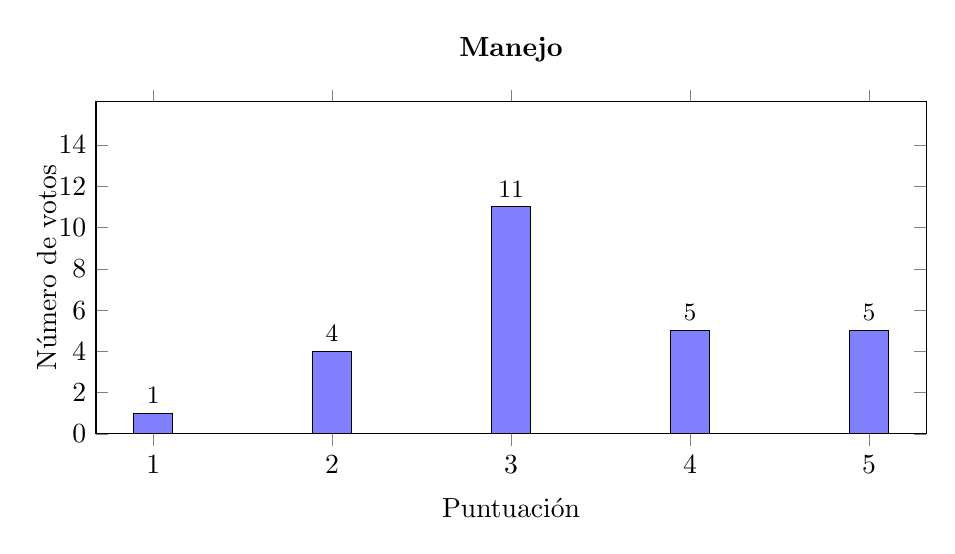
\begin{tikzpicture}
            \begin{axis}[
                tight grid bar,
                bar width=14pt,
                title={\textbf{Manejo}},
                ymin=0, ymax=14,
                ytick={0, 2, 4, 6, 8, 10, 12, 14},
                xtick={1, 2, 3, 4, 5},
                symbolic x coords={1, 2, 3, 4, 5}
            ]
            \addplot[fill=blue!50] coordinates {
                (1, 1) (2, 4) (3, 11) (4, 5) (5, 5)
            };
            \end{axis}
        \end{tikzpicture}
    \end{subfigure}\hfill
    \begin{subfigure}{0.49\textwidth}
        \centering
        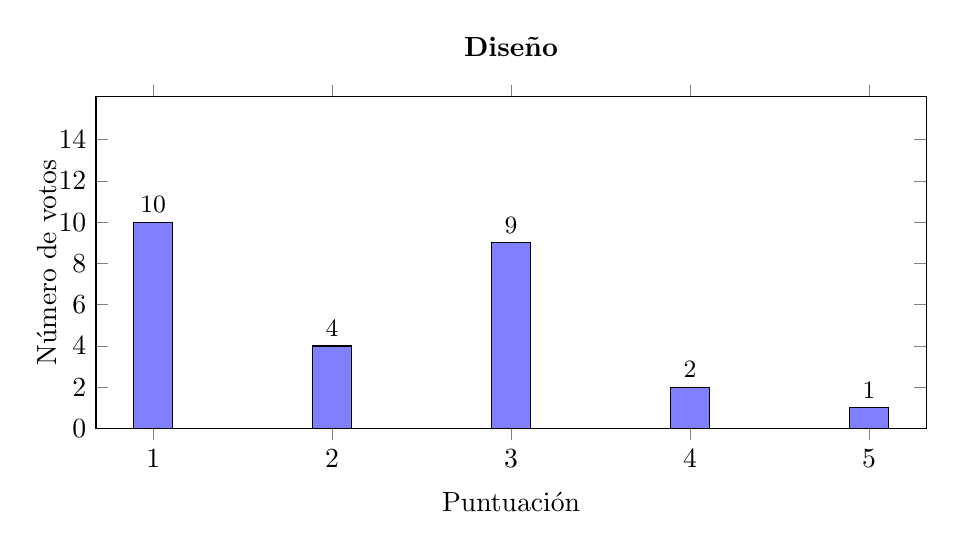
\begin{tikzpicture}
            \begin{axis}[
                tight grid bar,
                bar width=14pt,
                title={\textbf{Diseño}},
                ymin=0, ymax=14,
                ytick={0, 2, 4, 6, 8, 10, 12, 14},
                xtick={1, 2, 3, 4, 5},
                symbolic x coords={1, 2, 3, 4, 5}
            ]
            \addplot[fill=blue!50] coordinates {
                (1, 10) (2, 4) (3, 9) (4, 2) (5, 1)
            };
            \end{axis}
        \end{tikzpicture}
    \end{subfigure}

    \caption{Aspectos comunes}
    \label{fig:grid_common_aspects}
\end{figure}

Las cuatro gráficas de \ref{fig:grid_common_aspects} nos detallan cómo los usuarios sienten la interactividad con la aplicación. Esto nos puede ayudar a saber qué debemos cambiar respecto a la aplicación actual y qué podemos replicar y mejorar.

Podemos apreciar que a la mayoría de los usuarios no les desagrada la usabilidad. Con esto podemos intentar seguir un esquema de uso similar con el que cuenta la aplicación.

La accesibilidad parece seguir un patrón uniforme que crece conforme nos acercamos a valores que reflejan una menor accesibilidad. Lo que nos dice que la accesibilidad es un punto a mejorar necesitando crear un sistema intuitivo que no le genere fricción al usuario. 

El manejo es puntuado mayoritariamente con un valor medio, pero que decrece conforme nos acercamos a las mejores puntuaciones. Esto nos dice que necesitamos un sistema que ofrezca al usuario una distribución de los datos sencilla y entendible. 

Por último, el diseño no es puntuado muy alto, lo que nos dice que nuestro sistema deberá tener una mejora visual que sea atractiva para los usuarios.

\begin{figure}[htbp]
	\centering
	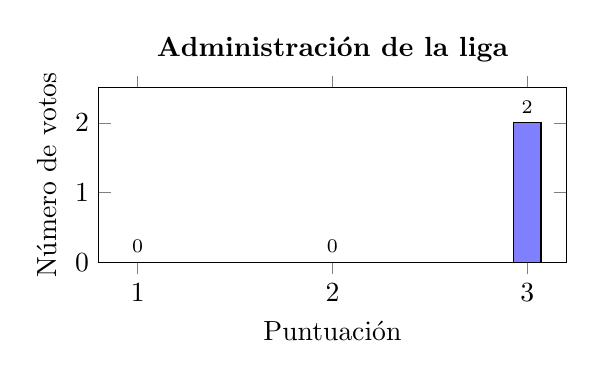
\begin{tikzpicture}
		\begin{axis}[title={\textbf{Administración de la liga}}, width=0.62\textwidth, ybar, bar width=10pt, height=3.8cm, ymin=0, ymax=2.5, xlabel={Puntuación}, ylabel={Número de votos}, xtick={1,2,3}, symbolic x coords={1,2,3}, nodes near coords, every node near coord/.append style={font=\scriptsize}]
		\addplot[fill=blue!50] coordinates {(1,0) (2,0) (3,2)};
		\end{axis}
	\end{tikzpicture}
	\caption{Valoración de la administración de la liga}
	\label{fig:admin_col}
\end{figure}

En la Figura \ref{fig:admin_col} vemos cómo la administración y gestión deportiva a través de la aplicación no es ni lo mejor ni lo peor. No habría que aplicar mejoras respecto a lo existente, pero podemos añadir nuevas funcionalidades que faciliten el trabajo de los administradores.

\begin{figure}[htbp]
	\centering
	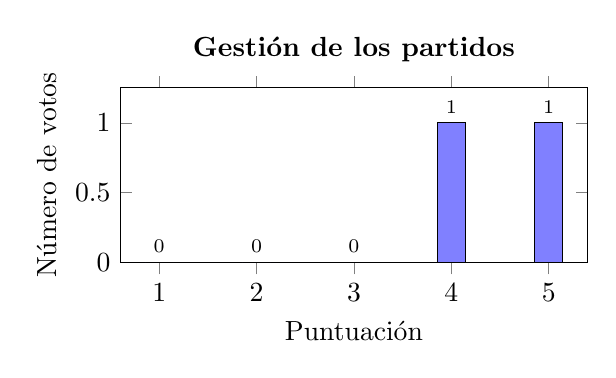
\begin{tikzpicture}
		\begin{axis}[title={\textbf{Gestión de los partidos}}, width=0.62\textwidth, ybar, bar width=10pt, height=3.8cm, ymin=0, ymax=1.25, xlabel={Puntuación}, ylabel={Número de votos}, xtick={1,2,3,4,5}, symbolic x coords={1,2,3,4,5}, nodes near coords, every node near coord/.append style={font=\scriptsize}]
		\addplot[fill=blue!50] coordinates {(1,0) (2,0) (3,0) (4,1) (5,1)};
		\end{axis}
	\end{tikzpicture}
	\caption{Valoración de la gestión de los partidos}
	\label{fig:referee_col_0}
\end{figure}

Según la Figura \ref{fig:referee_col_0}, la gestión de los partidos parece ser excelente. Aunque cabe recalcar que los árbitros utilizan diversas aplicaciones para gestionar los partidos: tanto para arbitrar un partido como para anotar los resultados. Por ello existe la necesidad de hacer un sistema unificado para todos los interesados.

\begin{figure}[htbp]
	\centering
	\begin{tikzpicture}[scale=0.75]
		\pie[text=legend, hide number, sum=auto, every pie/.style={font=\scriptsize}]{2/Tablet (2 votos)}
	\end{tikzpicture}
	\caption{Dispositivo utilizado para rellenar el acta}
	\label{fig:referee_col_1}
\end{figure}

La Figura \ref{fig:referee_col_1} nos confirma la necesidad del sistema multiplataforma al observar el uso de tablets por parte de los árbitros para rellenar el acta de los partidos.

\begin{figure}[htbp]
	\centering
	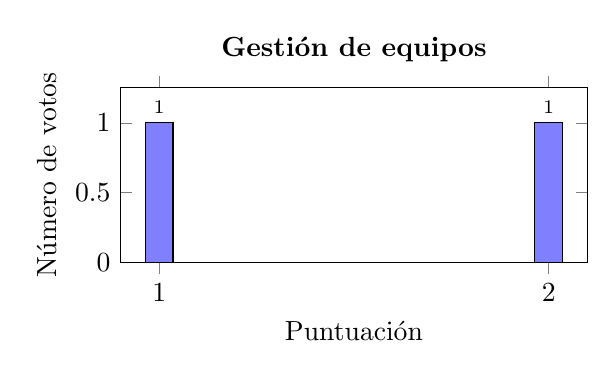
\begin{tikzpicture}
		\begin{axis}[title={\textbf{Gestión de equipos}}, width=0.62\textwidth, ybar, bar width=10pt, height=3.8cm, ymin=0, ymax=1.25, xlabel={Puntuación}, ylabel={Número de votos}, xtick={1,2}, symbolic x coords={1,2}, nodes near coords, every node near coord/.append style={font=\scriptsize}]
		\addplot[fill=blue!50] coordinates {(1,1) (2,1)};
		\end{axis}
	\end{tikzpicture}
	\caption{Valoración de la gestión de equipos}
	\label{fig:captain_col}
\end{figure}

En la Figura \ref{fig:captain_col} vemos como la opinión respecto a la gestión de equipos es muy baja. Esto nos lleva a deducir que puede ser interesante añadir funcionalidades para mejorar la interactividad y participación de los usuarios a la hora de gestionar los equipos deportivos.

\subsubsection*{Nota final y necesidad de un nuevo sistema}

\begin{figure}[H]
    
        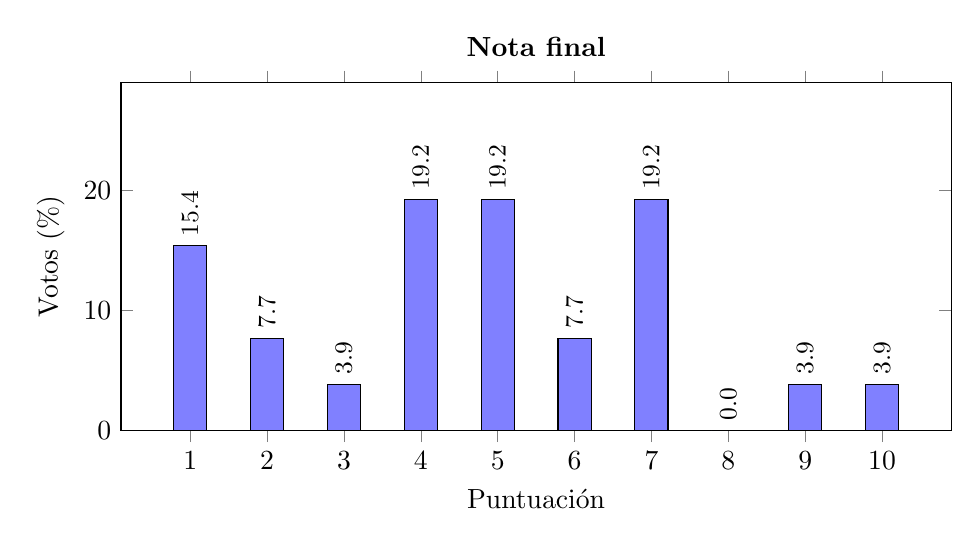
\begin{tikzpicture}
            \begin{axis}[
                title={\textbf{Nota final}},
                width=\textwidth,
                ybar,
                bar width=12pt,
                height=6cm,
                ymin=0, ymax=29,
                xlabel={Puntuación},
                ylabel={Votos (\%)},
                xtick={1, 2, 3, 4, 5, 6, 7, 8, 9, 10},
                symbolic x coords={1, 2, 3, 4, 5, 6, 7, 8, 9, 10},
                nodes near coords, 
                nodes near coords align={vertical},
                every node near coord/.append style={
                    font=\small,
                    rotate=90,
                    anchor=west,
                    /pgf/number format/.cd, fixed, fixed zerofill, precision=1
                }
            ]
            \addplot[fill=blue!50] coordinates {
                (1, 15.38) (2, 7.69) (3, 3.85) (4, 19.23) (5, 19.23) (6, 7.69) (7, 19.23) (8, 0.0) (9, 3.85) (10, 3.85)
            };
            \end{axis}
        \end{tikzpicture}
    
    \label{fig:col_final_result}
    \caption{Nota final}
\end{figure}
    
    \begin{figure}[H]
        \centering
        \begin{tikzpicture}
            \pie[text=legend]{
                96.15/Si, 3.85/No
            }
        \end{tikzpicture}
        \caption{¿Te gustaría una nueva aplicación que incluya nuevas y mejores funcionalidades?}
        \label{fig:col_new_app}
    \end{figure}
    \subsubsection*{Aspectos específicos}

\begin{figure}[htbp]
    \centering
    \hspace*{-0.15\textwidth}
    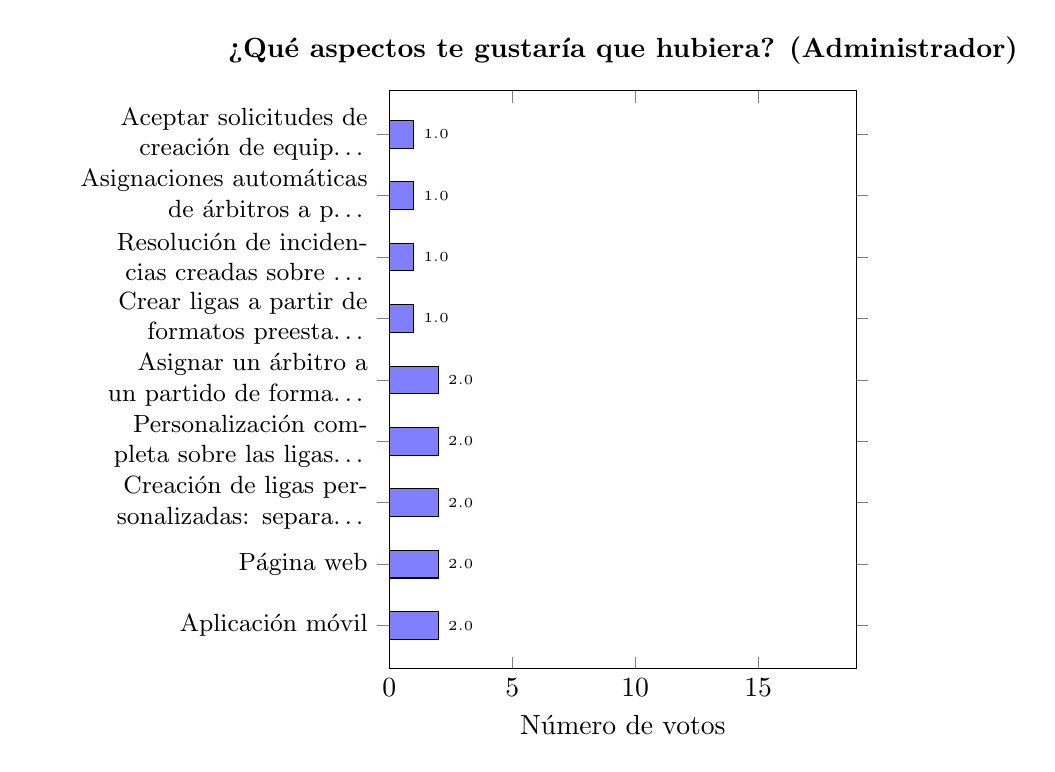
\begin{tikzpicture}
        \begin{axis}[
            title={\textbf{¿Qué aspectos te gustaría que hubiera? (Administrador)}},
            width=0.62*\textwidth,
            xbar,
            bar width=10pt,
            y=0.78cm,
            enlarge y limits={abs=0.55cm},
            xmin=0, xmax=19,
            xlabel={Número de votos},
            ytick={1,2,3,4,5,6,7,8,9},
            yticklabels={{Aplicación móvil}, {Página web}, {Creación de ligas personalizadas: separa\dots}, {Personalización completa sobre las ligas\dots}, {Asignar un árbitro a un partido de forma\dots}, {Crear ligas a partir de formatos preesta\dots}, {Resolución de incidencias creadas sobre \dots}, {Asignaciones automáticas de árbitros a p\dots}, {Aceptar solicitudes de creación de equip\dots}},
            yticklabel style={
                text width=4.2cm,
                align=right,
                font=\small
            },
            nodes near coords, 
            nodes near coords align={horizontal},
            every node near coord/.append style={
                font=\tiny,
                anchor=west,
                /pgf/number format/.cd, fixed, fixed zerofill, precision=1
            }
        ]
        \addplot[fill=blue!50] coordinates {
            (2, 1) (2, 2) (2, 3) (2, 4) (2, 5) (1, 6) (1, 7) (1, 8) (1, 9)
        };
        \end{axis}
    \end{tikzpicture}
    \label{fig:col_desired_functionalities_admin}
    \caption{Nuevas funcionalidades: Administrador}
\end{figure}

Vemos como los administradores buscan una mayor versatilidad y facilidad a la hora de poder gestionar la liga desde cualquier dispositivo. Una gestión amena que no genere fricción con el usuario.

\begin{figure}[htbp]
    \centering
    \hspace*{-0.15\textwidth}
    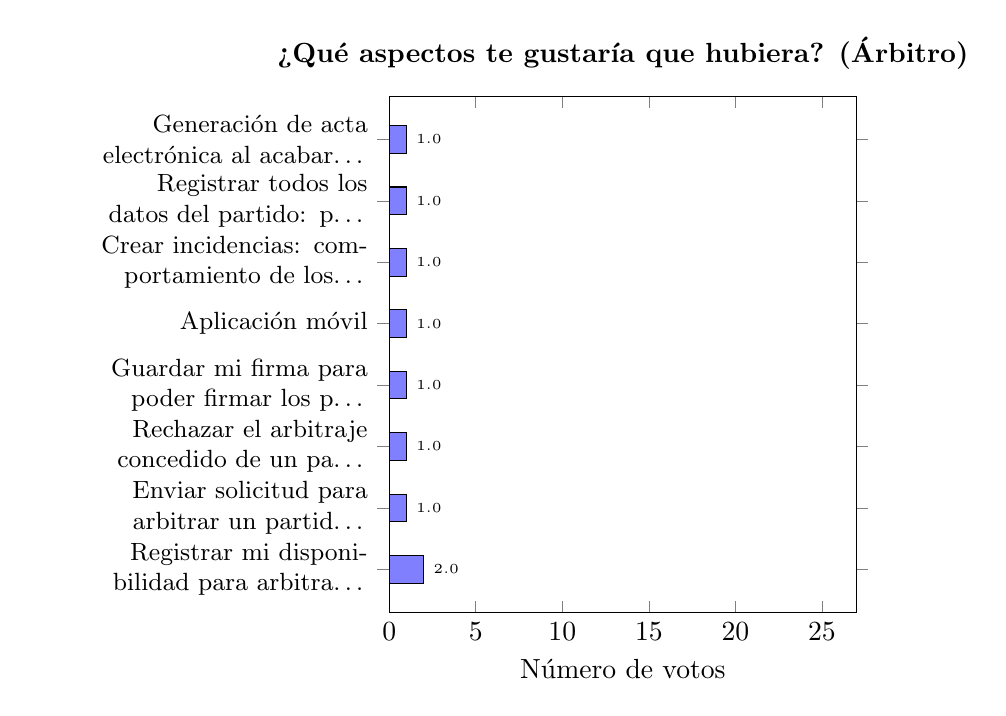
\begin{tikzpicture}
        \begin{axis}[
            title={\textbf{¿Qué aspectos te gustaría que hubiera? (Árbitro)}},
            width=0.62*\textwidth,
            xbar,
            bar width=10pt,
            y=0.78cm,
            enlarge y limits={abs=0.55cm},
            xmin=0, xmax=27,
            xlabel={Número de votos},
            ytick={1,2,3,4,5,6,7,8},
            yticklabels={{Registrar mi disponibilidad para arbitra\dots}, {Enviar solicitud para arbitrar un partid\dots}, {Rechazar el arbitraje concedido de un pa\dots}, {Guardar mi firma para poder firmar los p\dots}, {Aplicación móvil}, {Crear incidencias: comportamiento de los\dots}, {Registrar todos los datos del partido: p\dots}, {Generación de acta electrónica al acabar\dots}},
            yticklabel style={
                text width=4.2cm,
                align=right,
                font=\small
            },
            nodes near coords, 
            nodes near coords align={horizontal},
            every node near coord/.append style={
                font=\tiny,
                anchor=west,
                /pgf/number format/.cd, fixed, fixed zerofill, precision=1
            }
        ]
        \addplot[fill=blue!50] coordinates {
            (2, 1) (1, 2) (1, 3) (1, 4) (1, 5) (1, 6) (1, 7) (1, 8)
        };
        \end{axis}
    \end{tikzpicture}
    \label{fig:col_desired_functionalities_referee}
    \caption{Nuevas funcionalidades: Árbitro}
\end{figure}

Mientras que los árbitros se centran principalmente en que puedan especificar su disponibilidad y que el sistema actúe acorde.

\begin{figure}[htbp]
    \centering
    \hspace*{-0.15\textwidth}
    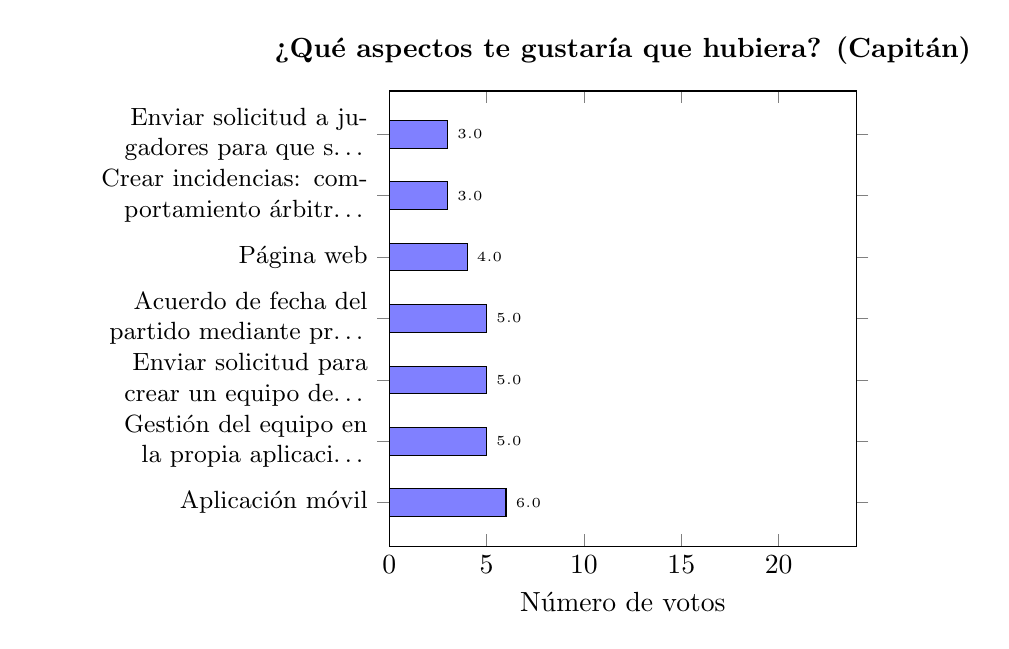
\begin{tikzpicture}
        \begin{axis}[
            title={\textbf{¿Qué aspectos te gustaría que hubiera? (Capitán)}},
            width=0.62*\textwidth,
            xbar,
            bar width=10pt,
            y=0.78cm,
            enlarge y limits={abs=0.55cm},
            xmin=0, xmax=24,
            xlabel={Número de votos},
            ytick={1,2,3,4,5,6,7},
            yticklabels={{Aplicación móvil}, {Gestión del equipo en la propia aplicaci\dots}, {Enviar solicitud para crear un equipo de\dots}, {Acuerdo de fecha del partido mediante pr\dots}, {Página web}, {Crear incidencias: comportamiento árbitr\dots}, {Enviar solicitud a jugadores para que s\dots}},
            yticklabel style={
                text width=4.2cm,
                align=right,
                font=\small
            },
            nodes near coords, 
            nodes near coords align={horizontal},
            every node near coord/.append style={
                font=\tiny,
                anchor=west,
                /pgf/number format/.cd, fixed, fixed zerofill, precision=1
            }
        ]
        \addplot[fill=blue!50] coordinates {
            (6, 1) (5, 2) (5, 3) (5, 4) (4, 5) (3, 6) (3, 7)
        };
        \end{axis}
    \end{tikzpicture}
    \label{fig:col_desired_functionalities_captain}
    \caption{Nuevas funcionalidades: Capitán}
\end{figure}

\begin{figure}[htbp]
    \centering
    \hspace*{-0.15\textwidth}
    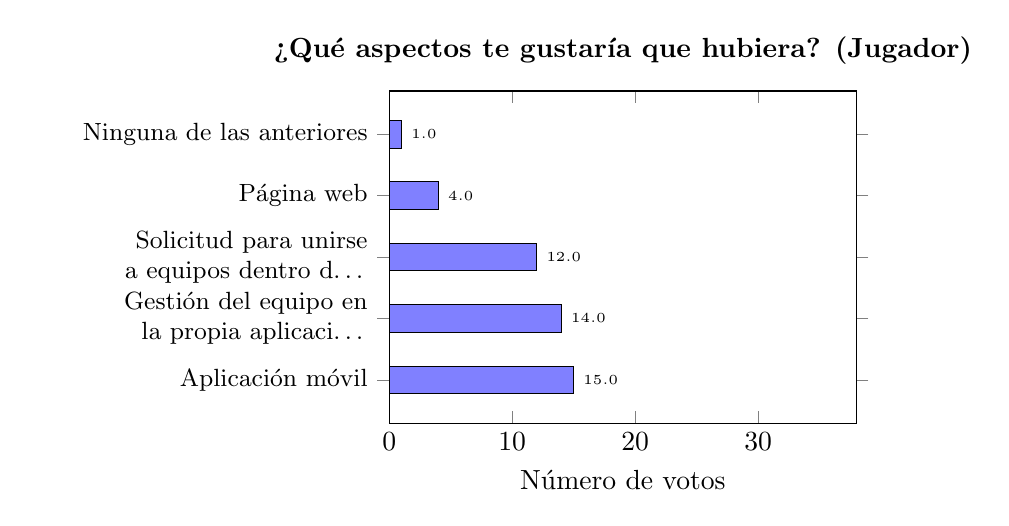
\begin{tikzpicture}
        \begin{axis}[
            title={\textbf{¿Qué aspectos te gustaría que hubiera? (Jugador)}},
            width=0.62*\textwidth,
            xbar,
            bar width=10pt,
            y=0.78cm,
            enlarge y limits={abs=0.55cm},
            xmin=0, xmax=38,
            xlabel={Número de votos},
            ytick={1,2,3,4,5},
            yticklabels={{Aplicación móvil}, {Gestión del equipo en la propia aplicaci\dots}, {Solicitud para unirse a equipos dentro d\dots}, {Página web}, {Ninguna de las anteriores}},
            yticklabel style={
                text width=4.2cm,
                align=right,
                font=\small
            },
            nodes near coords, 
            nodes near coords align={horizontal},
            every node near coord/.append style={
                font=\tiny,
                anchor=west,
                /pgf/number format/.cd, fixed, fixed zerofill, precision=1
            }
        ]
        \addplot[fill=blue!50] coordinates {
            (15, 1) (14, 2) (12, 3) (4, 4) (1, 5)
        };
        \end{axis}
    \end{tikzpicture}
    \label{fig:col_desired_functionalities_player}
    \caption{Nuevas funcionalidades: Jugador}
\end{figure}


Por último, tanto los capitanes como los jugadores buscan una mayor interacción con el sistema a la hora de gestionar los equipos.\subsubsection*{Preguntas abiertas}

\textbf{Otros aspectos}
\begin{itemize}
    \item Me gustaría que hubiera estado más adaptada al voleibol. Se nota que no está hecha para este deporte por el tema de la complicación de asignar una distinta puntuación a diferentes finales de partido o la falta de aparición de los puntos a favor y él contra en la clasificación. Además la asignación de los árbitros a los partidos es muy tediosa por tener que seleccionarlos uno a uno. Me gustaría también que se creará un calendario donde se viera más claramente cuando es cada partido y árbitro asignado.
    \item Yo solo querría que cada equipo gestionase su plantilla y que los resultados y la clasificación se actualice.
    \item Que se puedan visualizar los puntos de cada equipo una vez finalizado el partido. Que tenga la opción de notificaciones para los próximos partidos.
    \item Quiero, que los puntos se repartan eficientemente, porque la aplicación está programada para una liga de fútbol y no para puntualizar marcadores de vóley.
    \item Quiero que se puedan personalizar los propios equipos porque me parece una buena forma de participación.
\end{itemize}

\textbf{Problemas encontrados}
\begin{itemize}
    \item Me lío a veces al poner los resultados de los sets en cada apartado de los partidos.
    \item La aplicación que hay ahora solo se podía descargar en iPhone o era muy complicada de descargar.
    \item El desplegable de los grupos puede crear confusión, ya que no se modifica cuando has seleccionado otro deporte. Está predeterminado para el de fútbol. También en el apartado para ver los resultados deporte cada jornada (por fechas) solo está disponible los resultados de la primera jornada.
    \item Hay funciones que no terminan de cargar como  la bandeja de entrada o las notificaciones, va bastante lenta también.
    \item Me cuesta entrar porque no la veo nada práctica ni estética.
    \item El sistema de puntos suele ir mal, a veces diversos equipos han aparecido con otra cantidad de puntos que les corresponde a otros equipos.
    \item Hay errores en el tema de los partidos, por ejemplo hay partidos que no me salen de mi equipo o que aparecen como si no hubiesen pasado, pero ya han pasado varias semanas. No sé si es parte de la app o de quien mantiene la puntuación de cada partido, pero igual queda raro.
\end{itemize}
    